The closed loop system is shown in Figure~\ref{fig:hw_mass_system_type}.
\begin{figure}[H]
   \centering
   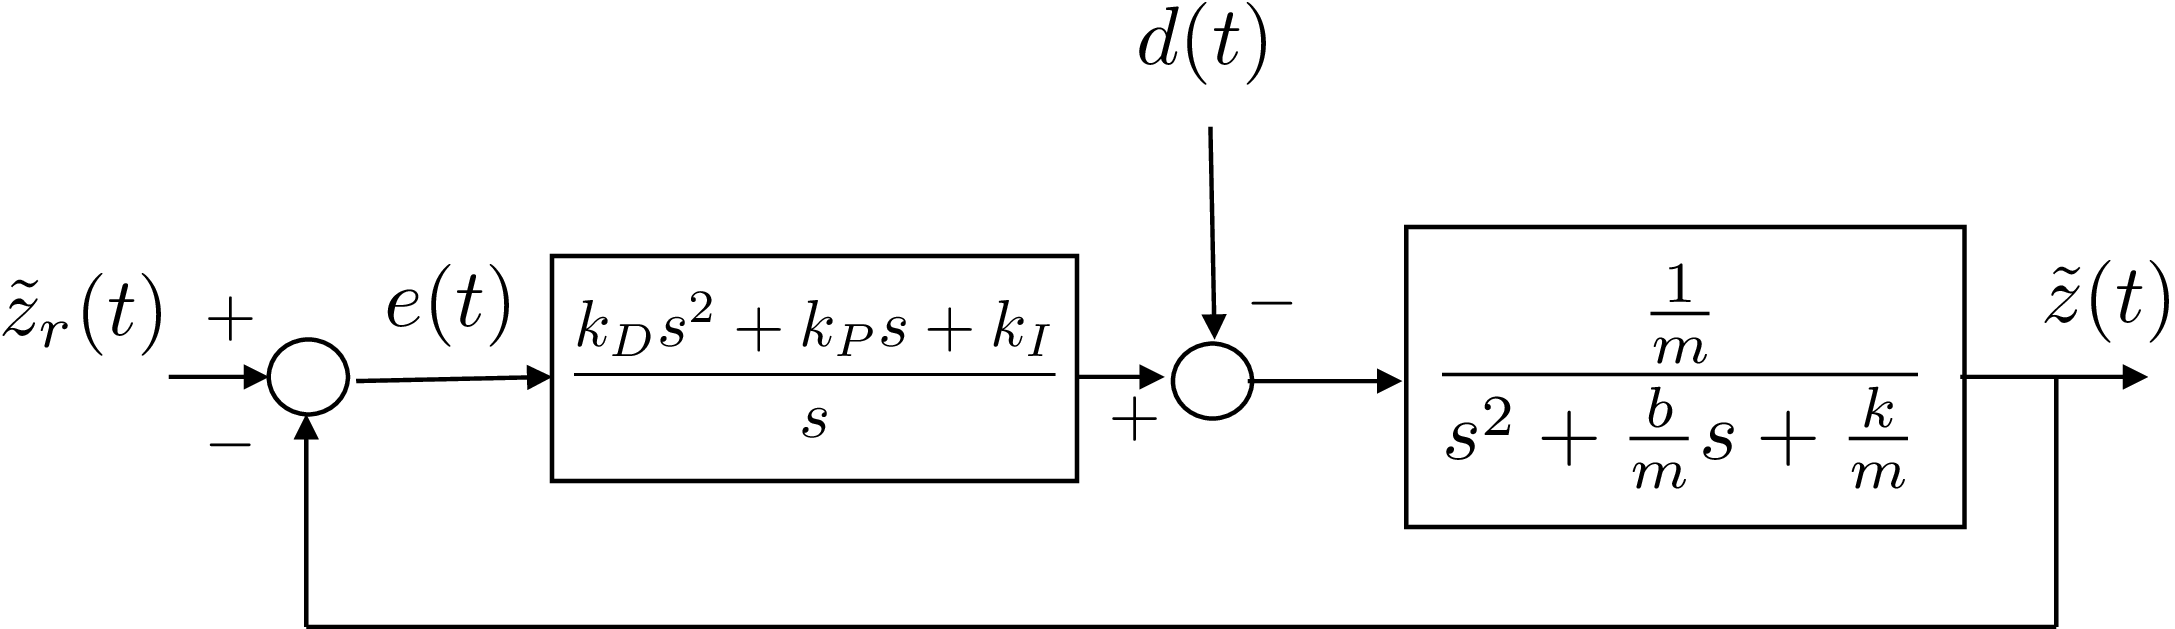
\includegraphics[width=0.7\textwidth]{6_design_studies/figures/hw_mass_system_type.pdf}
   \caption{Closed-loop system for problem mass-spring-damper system with PID control.}
   \label{fig:hw_mass_system_type}
\end{figure}
Without the integrator, the open-loop transfer function is given by
\[
P(s)C(s) = \left(\frac{\frac{1}{m}}{s^2 + \frac{b}{m}s + \frac{k}{m})}\right)\left(k_D s + k_P\right).
\]
The system has no free integrators and is therefore type~0, which, from Table~\ref{table:system_type} implies that the tracking error when the input is a step is 
\[
\lim_{t\to\infty}e(t) = \frac{1}{1+M_p} = \frac{1}{1+\lim_{s\to 0} P(s)C(s)} = \frac{k}{k+k_P}.
\]
The tracking error when the input is a ramp, parabola, or higher order polynomial, is $\infty$, meaning that $z(t)$ and $z_r(t)$ diverge as $t\to\infty$.

With the integrator, the open loop transfer function is
\[
P(s)C(s) = \left(\frac{\frac{1}{m}}{s^2+\frac{b}{m}s+\frac{k}{m})}\right)\left(\frac{k_D s^2 + k_Ps + k_I}{s}\right).
\]
which has one free integrator and is therefore type~1. Therefore, from Table~\ref{table:system_type} the tracking error when the input is either a step is zero, and the tracking error when the input is a ramp is
\[
\lim_{t\to\infty}e(t) = \frac{1}{M_v} = \frac{1}{\lim_{s\to 0} sP(s)C(s)} = \frac{k}{k_I}.
\]
The tracking error when the input is $t^2$ or a higher order polynomial, is $\infty$.

For the input disturbance, the transfer function from $D(s)$ to $E(s)$ is given by
\[
E(s) = \frac{P(s)}{1+P(s)C(s)}D(s).
\]
Without the integrator, and when $D(s)= \frac{A}{s^{q+1}}$, the steady state error is given by
\begin{align*}
\lim_{t\to\infty} e(t) &= \lim_{s\to 0} \frac{P}{1+PC}\frac{A}{s^q} \\
&= \lim_{s\to 0} \frac{\left(\frac{\frac{1}{m}}{s^2+\frac{b}{m}s+\frac{k}{m}}\right)}{1+\left(\frac{\frac{1}{m}}{s^2+\frac{b}{m}s+\frac{k}{m}}\right)\left(k_Ds+k_P\right)}\frac{A}{s^q} \\
&= \lim_{s\to 0} \frac{\frac{1}{m}}{\left(s^2+\frac{b}{m}s+\frac{k}{m}\right)+\frac{1}{m}\left(k_Ds+k_P\right)}\frac{A}{s^q} \\
&= \lim_{s\to 0} \frac{1}{k+k_P}\frac{A}{s^q} \\
&= \frac{A}{k+k_P},
\end{align*}
if $q=0$.  Therefore, to an input disturbance the system is type~0.  The steady state error when a constant step of size $A$ is placed on $d(t)$ is $\frac{A}{k+k_P}$.  

With the integrator, and when $D(s)= \frac{A}{s^{q+1}}$, the steady state error is given by
\begin{align*}
\lim_{t\to\infty} e(t) &= \lim_{s\to 0} \frac{P}{1+PC}\frac{A}{s^q} \\
&= \lim_{s\to 0} \frac{\left(\frac{\frac{1}{m}}{s^2+\frac{b}{m}s+\frac{k}{m}}\right)}{1+\left(\frac{\frac{1}{m}}{s^2+\frac{b}{m}s+\frac{k}{m}}\right)\left(\frac{k_Ds^2+k_Ps+k_I}{s}\right)}\frac{A}{s^q} \\
&= \lim_{s\to 0} \frac{s\frac{1}{m}}{s\left(s^2+\frac{b}{m}s+\frac{k}{m}\right)+\frac{1}{m}\left(k_Ds^2+k_Ps+k_I\right)}\frac{A}{s^q} \\
&= \lim_{s\to 0} \frac{\frac{1}{m}}{s\left(s^2+\frac{b}{m}s+\frac{k}{m}\right)+\frac{1}{m}\left(k_Ds^2+k_Ps+k_I\right)}\frac{A}{s^{q-1}} \\
&= \lim_{s\to 0} \frac{1}{k_I}\frac{A}{s^{q-1}} \\
&= \frac{A}{k_I},
\end{align*}
if $q=1$.  Therefore, to an input disturbance the system is type~1.  The steady-state error when $d(t)$ is a constant step is zero, and the steady-state error when $d(t)$ is a ramp of slope of size $A$ is $\frac{A}{k_I}$.  
